\chapter{Deep Learning}
\label{cha:dl}

Machine learning methods are used widely for regression and classification problems. Contemporary companies in order to keep up with the pace of customers expectations rely heavily on such algorithms. They require human intervention to learn. Which is possible for relatively small data sets, but gets extremely complicated or even impossible for larger ones. \textbf{Deep learning (DL)}, however, solves that issue by eliminating the need of human supervision by automating feature extraction. These algorithms can leverage from labeled data sets but do not require them to function. Together with the scalability, DL methods are by far superior to any other Artificial Inteligence solutions. This sections gives an insight of how \textbf{Deep Neural Networks (DNN)}, which are the core of DL, are created.


\section{Deep Neural Network Architecture}
\label{sec:dnn-arch}

\subsection{Neuron}
\label{sub:neuron}

Neuron is the most elementary part of the \textbf{Artificial Neural Network (ANN)}. The idea behind it was to emulate the behaviour of its biological counterpart. It consists of set of inputs $x_1, x_2, ..., x_n$ connected with digital synapses. Each of this connections is given a weight $w_1, w_2, ..., w_n$ representing an importance of the receptive inputs to the output. The output of neuron is determined by the \textbf{activation function} $\phi(x)$, which is described in more detail in the next section (\ref{sub:activation-function}). Where $x$ is the weighted sum of $\sum_j {x_j}{w_j}$ offset by bias $b$. To simplify, the weighted sum can be expressed as a dot product $x \cdot w$.

\begin{figure}[h]
    \centering
    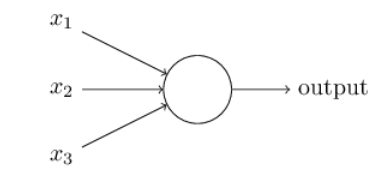
\includegraphics[width=8cm]{img/Perceptron.png}
    \caption{A neuron. Source \cite{NNandDL}}
    \label{fig:neuron}
\end{figure}

\subsection{Activation Function}
\label{sub:activation-function}

Every neuron in network, except inputs, consists of an activation function. In simple terms, it takes sum of weighted inputs and returns a value which tells how strong the neuron fires. In other words, the higher the activation function return, the stronger influence it has on the next layer. The return is usually within the range $[0, 1]$. Examples of activation functions are: 
\begin{itemize}
    \item Threshold \hspace{5pt}
        $\phi(x) = 
        \begin{cases}
            1 & x \ge 0 \\
            0 & x<0
        \end{cases}$
    \item Sigmoid \hspace{5pt}
        $\phi(x) = \frac{1}{1+e^{-x}}$
    \item Hyperbolic Tangent (tanh) \hspace{5pt}
        $\phi(x) = \frac{1-e^{-2x}}{1+e^{-2x}}$
    \item Rectifier Linear Unit (ReLU) \hspace{5pt}
        $\phi(x) = max(x, 0)$
\end{itemize}

The most commonly used is undoubtedly the \emph{ReLU}, which was proposed and researched by \emph{Xavier Glorot et al.} \cite{DeepSparseReNN}. It allows a network to easily obtain a sparse representation, which has numerous advantages and also mostly resembles neurobiological structures. Human brain is hypothesized to have 95\% to 99\% sparsity.